\documentclass[senior,final,11pt]{iscs-thesis}
\usepackage[dvipdfmx]{graphicx}
\etitle{A Method of Improving QoS:  Explorations of the Possibility of Function Combinations in Service Compositions}
\jtitle{品質改良のアプローチ:機能のぶれを許すサービス合成}
%
\eauthor{Ziyuan Wang}
\jauthor{王子源}
\esupervisor{Shinichi Honiden}
\jsupervisor{本位田真一}
\supervisortitle{Professor} % Professor, etc.
\date{February 9, 2016}
%-------------------
\begin{document}
\begin{eabstract}
There is a growing need for web service providers to develop customised and flexible web services as quick as they can. One way to satisfy this demand is to utilise service compositions, which provide a method of consolidating several services to a richer service. Because of the uncertainty in the feasibility of the functional and QoS requirements, it is not guaranteed that service compositions succeed with suitable solutions.

One way to satisfy the given requirements is to control the given two kinds of requirements. There have been studies on methods of optimising the QoS with fixed functional requirements. However, the search space in that case is limited, which would possibly not include service compositions with better QoS whose functions are slightly different from the required one. Therefore, I focus on the possibility of improving the QoS by compromising on functions or exploring the possibility of function combinations. This enables better advice of service compositions to users. In this article, I propose a method of efficiently searching different possibilities to support users to balance functional requirements and QoS requirements.
\end{eabstract}
\begin{jabstract}
近年,ウェブサービスプロバイダーにとって,ユーザーの好みに合わせた,柔軟なウェブサービスを短時間で作る必要性が増してきている.そのために,よく使われている手法として,複数のサービスを一つにまとめてより高機能なサービスを作るサービス合成と呼ばれる手法がある.サービス合成において,入力として受け取る機能や品質に関する要求を必ず満たせるとは限らないという問題がある.

機能と品質の両方を達成するために既存研究で提案されている手法として,その片方を固定して保証し,もう片方を最適化するというものがある.しかし,この手法では,機能を固定するために,探索空間が限られているため,
要求された機能に妥協を許した場合に品質が大きく高まるような合成を見逃す可能性がある.よって,本論文では,ユーザーが高品質の合成を見つけることがより容易になるよう,機能を妥協し,要求された機能と少しのぶれを許すことで探索空間を増やすことによるQoSの最適化の可能性について議論した.本論文では,ユーザーが機能要求と品質要求のバランスを取れるように効率的に様々な合成の可能性を探索する手法を提案した.

\end{jabstract}
\maketitle

\begin{acknowledge}
I appreciate Prof. Ishikawa's help in improving the structure of the paper.
\end{acknowledge}

\frontmatter 
\tableofcontents
%\listoffigures
%\listoftables 
%\lstlistoflistings
%-------------------
\mainmatter 

\chapter{INTREODUCTION}
Web service, service-based system, and service composition are significant.
%ws 基于service的系\UTF{7EDF} 和service合成是很重要的
A lot of existing studies on QoS-aware service composition.
%介\UTF{7ECD}下上面提到的几个名\UTF{8BCD},\UTF{8BA8}\UTF{8BBA}下它\UTF{4EEC}的来\UTF{9F99}去脉 
Fixed functional requirements -> may lose potential improvement of QoS, difficulty for users to properly define the functional requirements because of uncertainty of the feasibility of requirements given available services
%\UTF{8BA8}\UTF{8BBA}它\UTF{4EEC}的不好,固定fun\UTF{5BFC}致没法找到更好的qos
Tis paper ... (summary of the remainder).
%本文的主\UTF{9898},干了什\UTF{4E48}。
Chapter 2 describes ... Chapter 3...
%\UTF{6BCF}一章做了什\UTF{4E48}%
\section{Background}
%背景
\section{Goals}
%我\UTF{4EEC}的目的
\section{Contributions}
%本文的\UTF{8D21}献
\cite{4065825}. 
%-------------------
\chapter{Preliminary}%1-18------------------------
%已有的定\UTF{4E49}%
%Existing definitions.
~~~~This section defines some key terms of formal research of the service composition that I continue to use in this paper.
\section{Service}
%所\UTF{8C13}service,就是功能可重\UTF{590D}利用的
~~~~A service S is a reusable system that provides functionalities which are documented in a service description. This description defines a 5-tuple {\em IOPEQ = (S.I, S.O, S.P, S.E, S.Q)} where {\em S.I, S.O} are abbreviated from the required inputs and outputs of the S, {\em S.P, S.E} are the preconditions and effects which denote the necessary condition of utilising S and the consequence after running S, and {\em S.Q} is the set of the QoS attributes of the S. \\
%\UTF{5173}于service,一般分成service(instance)和service task\UTF{4E24}\UTF{79CD}\UTF{8BF4}法。service task
~~~~In this paper, {\em S.P, S.E} are ignored therefore a service S is modelled only with 3-tuple {\em IOQ = (S.I, S.O, S.Q)}.
%service (instance) and service task
%IOPEs -> modelled only with IO in this paper
%+ 
%Q
\section{QoS}
~~~~QoS is abbreviated from quality-of-service, that is, quality apart from the functionality the service can provides, such as the price, the execution time and the reliability of the service.
The S.Q of a service S is consist of a number of QoS attributes which is normalized between 0 and 1, with 0 being the worst and 1 being the best.
%multi-criteria
%normalized

\section{Service Compliance}
%Connectivity between two services
~~~~If there exists an output {\em o} $\in$ {\em S.O} of a service S is compatible with an input of {\em i}  $\in$ {\em S'.I} of another service S', we say there is a service link between S and S', written as S $\to$ S'. That is, the type of {\em o} is the same or a subtype of i. \\
~~~~In this paper, a service is constrained to has only one input and one output, therefore S $\to$ S' iff:
\begin{center}
{\em o} = {\em S.O} ,  {\em i} = {\em S'.I} ,  {\em o} $\in$ {\em i}
\end{center}

\section{I/O Plug-in match}
%我\UTF{4EEC}可以根据input或者output的兼容\UTF{5173}系来\UTF{7ED9}\UTF{4E24}个差不多功能的
~~~~Two functionality similar services, in this paper that denotes they are in the same task, may have two relations, defined as follow.\\
~~~~An Input Plug-in match $\sqsubseteq$ is a S $\times$ S relation that holds iff:
\begin{center}
S $\sqsubseteq$ S'  $\Leftrightarrow$ {\em S.I} $\in$ {\em S'.I}
\end{center}
~~~~In this paper, S $\sqsubseteq$ S' is referred to as S' is input-stronger than S, and S is input-weaker than S'.\\
~~~~An Output Plug-in match $\subset$ is a S $\times$ S relation that holds iff:
\begin{center}
S $\subset$ S' $\Leftrightarrow$ {\em S.I} $\in$ {\em S'.I}
\end{center}

In this paper, S $\subset$ S' is referred to as S' is output-stronger than S, and S is output-weaker than S'.\\


\section{Workflow}
~~~~A workflow is a sequence of two or more linked services. The functions of a workflow depend on function combinations that consist of the input parameter of the workflow's first service and the output parameter of the workflow's last service. A workflow template contains service tasks instead of actual services. A task is characterised as an abstract functionality which can be replaced by an actual service. There are generally two ways to assign services to a task, one is to compare the functions of the services with the functional requirements of the task. The other is to collect services depend on documents such as service description, which are usually distributed with the service by provider. Finally, each task is assigned with a set of services which meet the functional requirements of the task.

Selection algorithms receive a workflow template with fixed functional requirement and a dozens of services, and select for each task of one or more services which guarantee the obtained workflow's QoS are optimised, then return the obtained workflow as an output.

%Figure 1 shows an example workflow template and a possible service selection. may be add after
%Functional requirements: ぶれなし (existing)


\section{QoS optimization}
%this time single-objective

%-------------------
\chapter{Extended Composition Problem}: Proposal1

%motivation again
%
%ぶれありのcomposition problem定義
%def. 何段階ずれてもよい
(actually, not so meaningful to use too weak services)


\chapter{Algorithm for Extended Composition Problem}: Proposal 2

\subsection{Functionality Graph}
From [Wagner'11]
def.
algorithm

\subsection{Skyline}
def.
algorithm

\subsection{Naive Algorithm}
%for all 機能のぶれ (same, IN_one_weak-OUT_same, IN_same-OUT_one_weak, ...)
 % solve

\subsection{Algorithm}%\UTF{641E}个牛逼的名字
% ぶれの探索順序をソート -> ランダム,強い順,弱い順
%for all 機能のぶれ (same, IN_one_weak-OUT_same, IN_same-OUT_one_weak, ...)
 % if (これまでに求めた最適解が,今回も使えるなら)
 %   それをreturn
 % solve(前回の探索結果) // さらに再利用?

\chapter{Experiments}

\section{Implementation}
Implemented with Python.

\section{Extended Composition Problem}
Evaluation of Proposal 1\\
How QoS can be improved by allowing compromise in functional requirements?
\[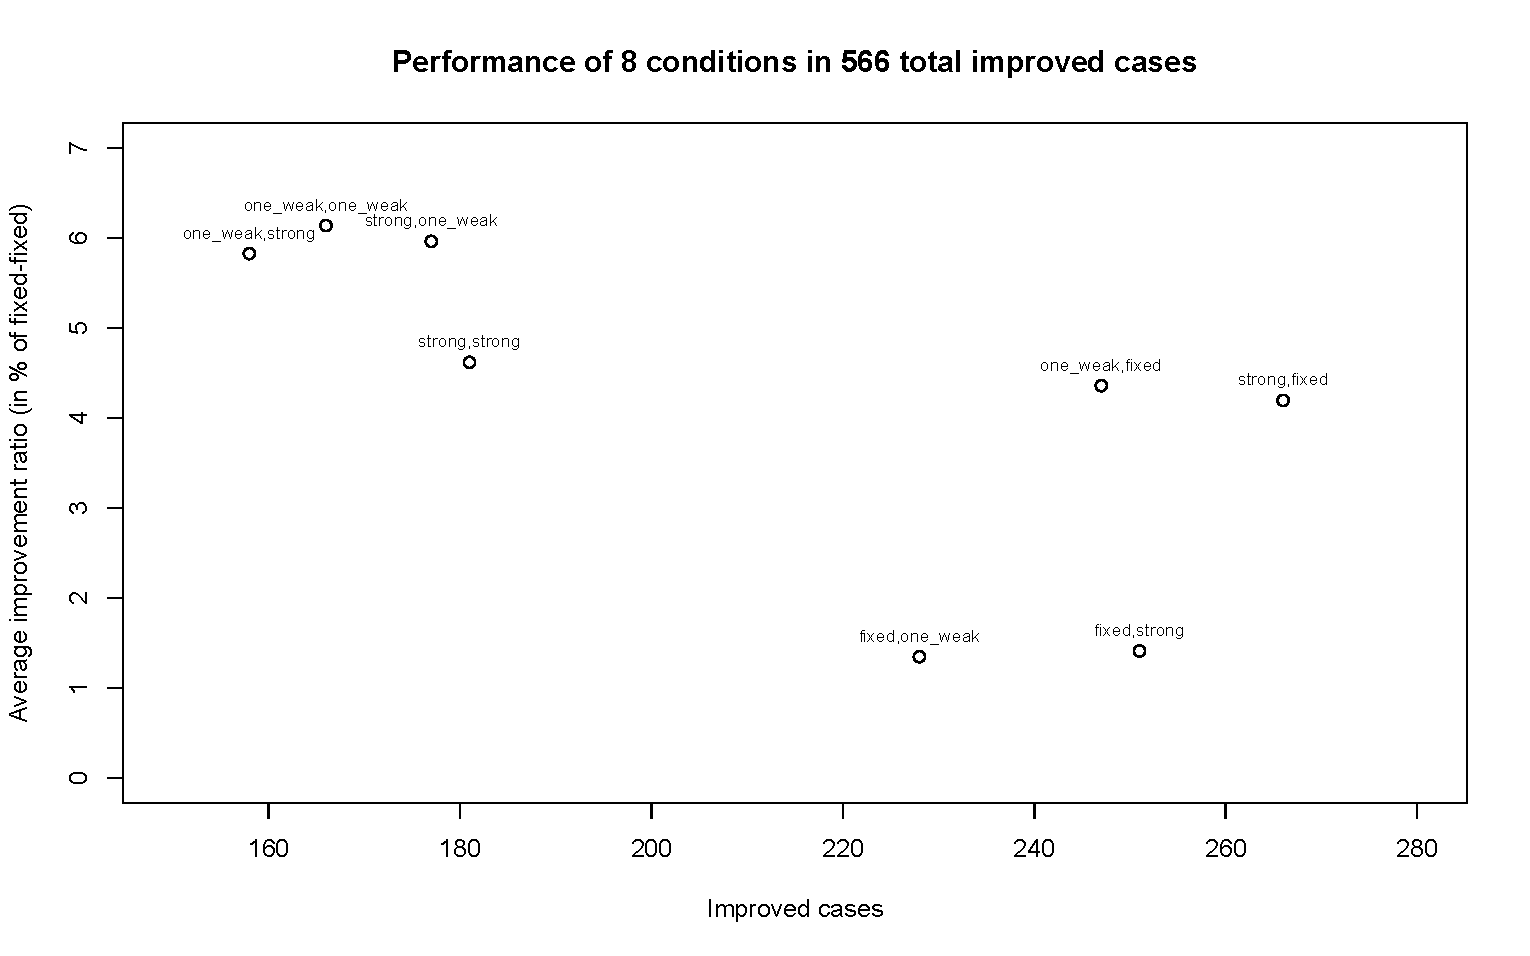
\includegraphics[width=13cm]{eval2.pdf}\]

\section{Algorithm}
Evaluation of Proposal 2\\
How fast can the proposed algorithm solve the extended problem?\\
- with skyline vs. without skyline\\
Fig. x depicts the relationship of step numbers between full search and skyline algorithm.
\[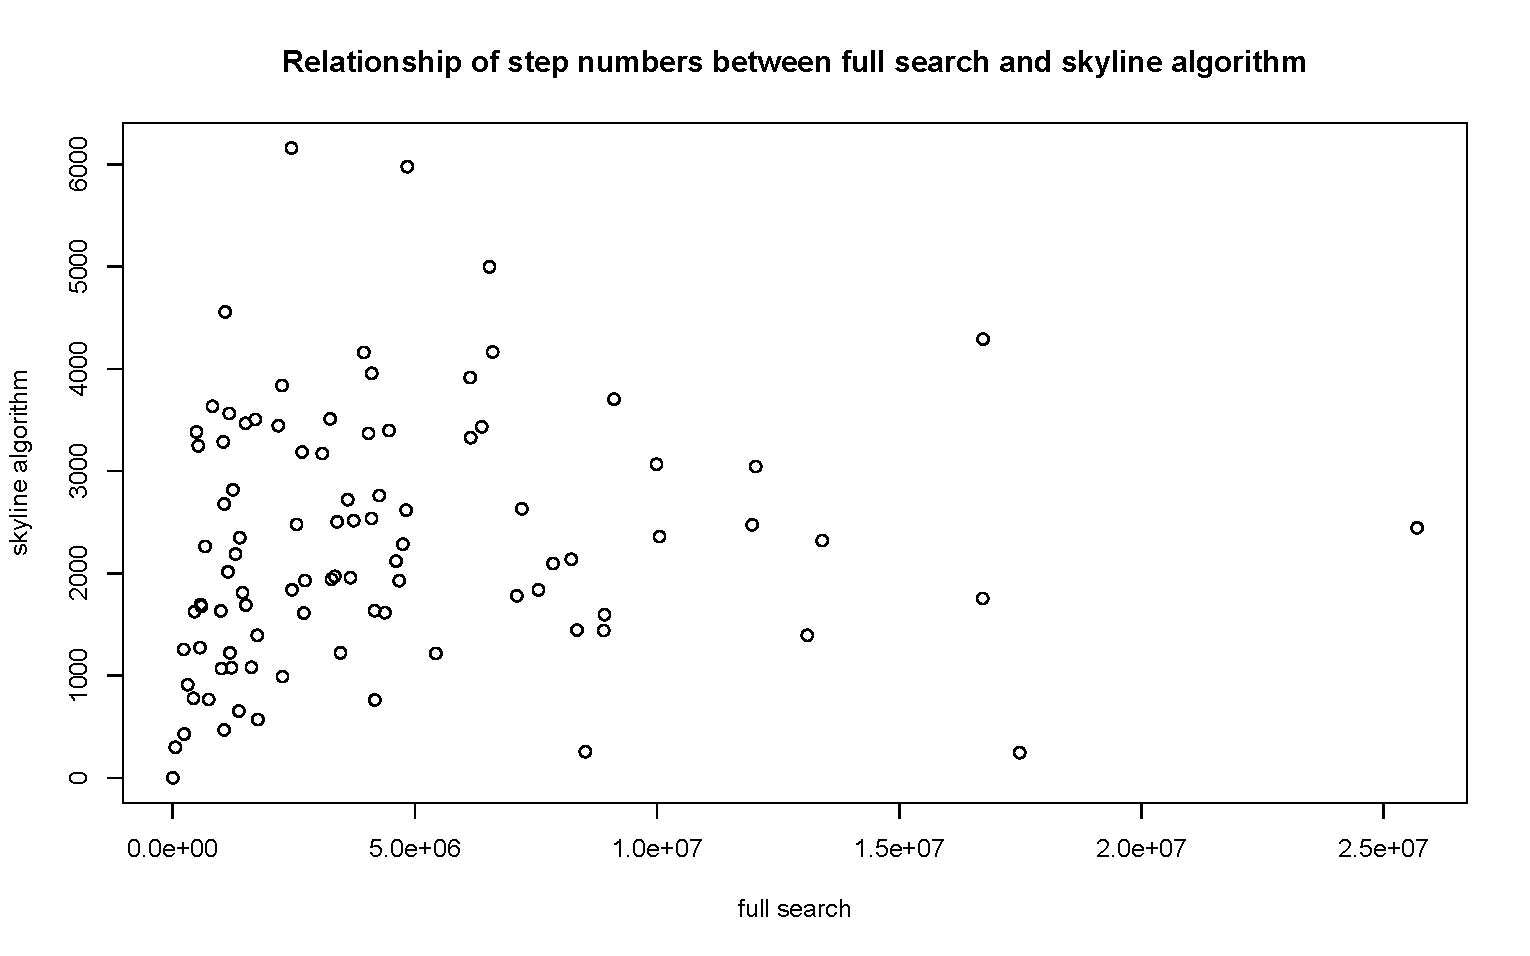
\includegraphics[width=13cm]{eval1.pdf}\]
By further calculation, the correlation between them is measured to be 0.1814083, which demonstrate the existence of weak correlation.

- with skyline vs. proposed algorithm with skyline

\chapter{Discussion}

% related work can come here

\subsection{Proposal}
The extended problem should be significant because in the experiment

The proposed algorithm made good improvement because in the experiment 

% if difficult, combine to the experiment chapter

\subsection{Future Work}
- QoS constraints
- adaptive


\chapter{Conclusion}

%-------------------
\bibliographystyle{plain} 
\bibliography{myref} 
%-------------------
\end{document}
